Adventures in Recreational Mathematics: Volume I.

Salutations!

This is the first of a new series in \emph{The Librarian }-- each issue,
we will discuss a different mathematical field or distinct problem
chosen due to their great utility, their results being intriguing or,
quite simply, they are enjoyable to play around with.

Each article will be written by one of (or both of) \emph{Isky Mathews
\& Benedict Randall Shaw}, discussing subjects we believe that others
will find stimulating as we do on a daily basis.

Also, for those interested, at the end of each article we will leave a
thematic problem of variable difficulty whose solutions should be
emailed to either one of the authors. Mathematics can be confusing, it
can be surprising but it can also be a lot of fun; this is what
\emph{Adventures in Recreational Mathematics }aims to tap into!

For our first issue, we will be considering \emph{tiling. }Tiling is the
study of how sets of polygons fit together on \emph{the plane, }to see
whether they \emph{tile }(i.e.~can be placed together in such a way that
there are no gaps left across the plane) and to learn if there are
geometric principles which could allow us to determine whether these
sets can tile the plane or not. Formally, we are concerned with covers
of the Euclidean plane formed by countable sets of \emph{closed sets
}such that they intersect only on their boundaries. We begin with the
simplest form of tiling, \emph{regular }tessellations, where the tiling
is \emph{translationally similar }over arbitrary distances and uses only
identical \emph{regular polygons -- monohedral }examples of this (ones
using only a single \emph{prototile}) are very well known.

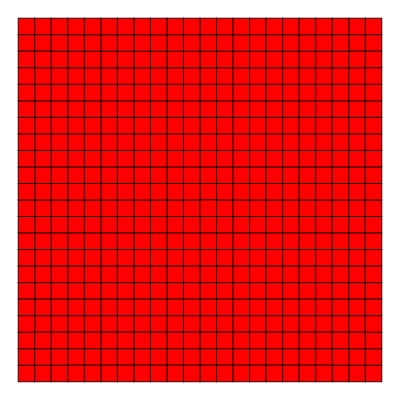
\includegraphics{image_0.png}
\includegraphics{image_1.png}
\includegraphics{image_2.png}

We would also say that these tilings are \emph{isogonal }or
\emph{vertex-transitive, }i.e.~every vertex has an identical arrangement
of tiles around it, and also that they are \emph{edge-to-edge }tilings,
since a given edge of each tile touches no more than one edge from
another tile.

Perhaps unsurprisingly, it is trivial to prove that for \(∀ n∈R, n<2\)
there is an irregular \(n\)-gon which tessellates. This can be seen by
constructing the shapes below:

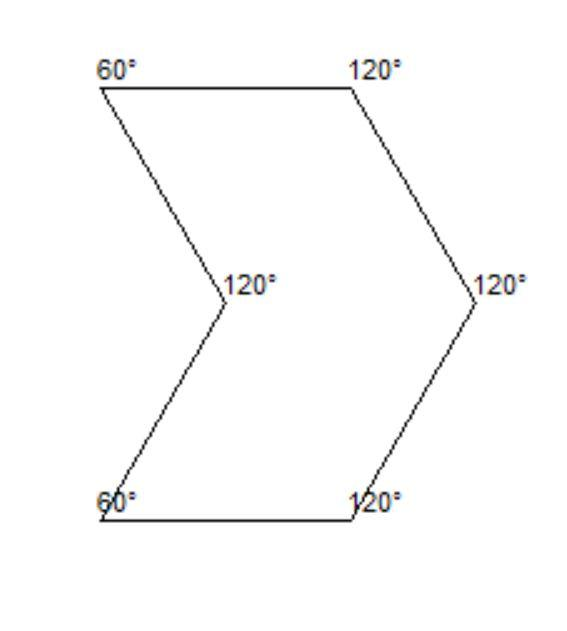
\includegraphics{image_3.jpg}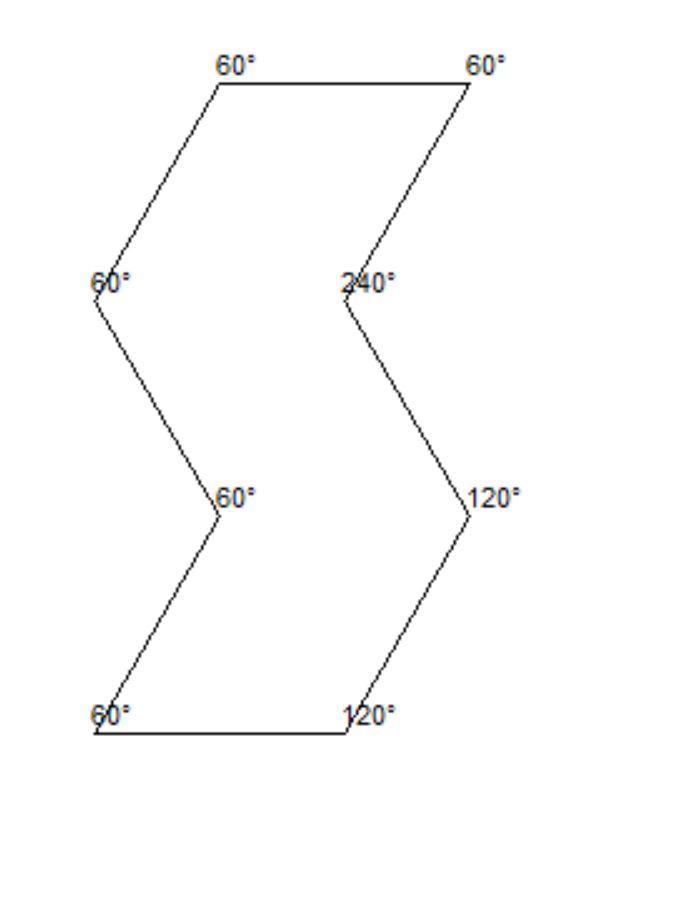
\includegraphics{image_4.jpg}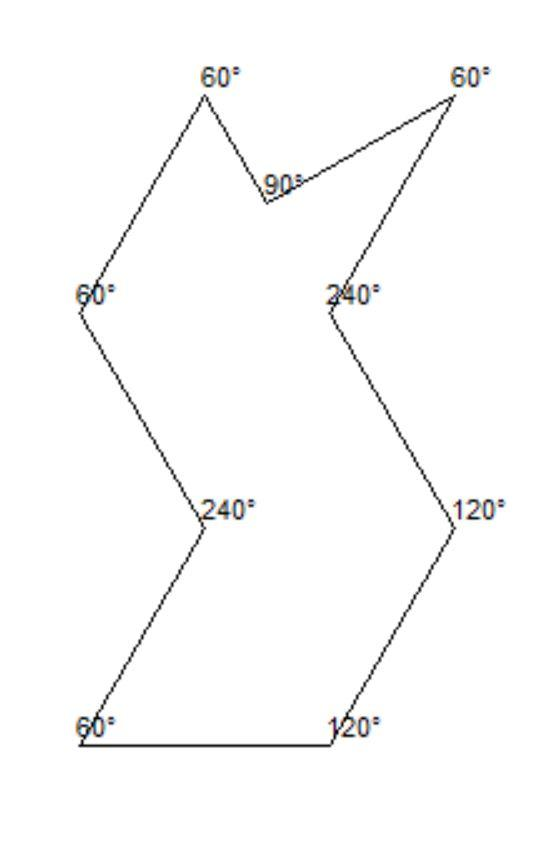
\includegraphics{image_5.jpg}

The leftmost figure displays a tessellating hexagon and by adding
another pair of sides on top, we get the second figure (a tessellating
octagon). We can continue adding pairs like this to get tessellating
-gons for even. The third figure shows a way of making these figures odd
sided, while retaining tessellation (the forked parts can interlock with
two forked parts of other tiles). Thus, you can construct all even and
odd numbered -gons for using this method!

There are, as you can imagine, many other ways of constructing
tessellating -gons and in fact many ways of tiling them. If we allow
ourselves to tile on a plane with \emph{negative curvature }(commonly
known as the \emph{hyperbolic plane}), then you can have significantly
more tilings -- for example, in the Euclidean plane we tile 6
equilateral triangles around a point but in the hyperbolic plane you can
have all the way to an infinite number of triangles around a point! This
geometry requires greater examination on its own, but that is not the
focus of the article.

There are also \emph{semiregular tilings}, those that are made up of
more than one tile but are still periodic, such as this lovely tiling
using squares, hexagons and dodecagons:

\begin{figure}[htbp]
\centering
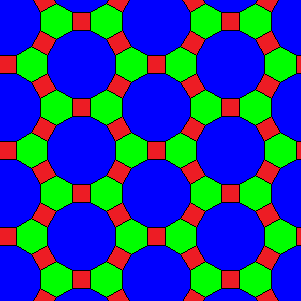
\includegraphics{image_6.png}
\caption{}
\end{figure}

However, these are all quite trivial examples and concepts. There are
numerous, seriously difficult problems: the so-called \emph{tiling
problem, }the \emph{five-fold symmetry problem }and understanding
\emph{Heesch's Problem }are just a few.

The \emph{tiling problem} is to create an algorithm or set of principles
to determine whether a \emph{prototile set} tiles, in finite time. A
form of this was first proposed by the philosopher and mathematician Hao
Wang in 1961, after discovering sets of \emph{aperiodic} tiles called
\emph{Wang tiles. }An \emph{aperiodic tiling }is one that has no
arbitrary distance \emph{translational symmetry }and \emph{aperiodic
tiles }are those that can \emph{only }tile the plane aperiodically. The
colours on each side of a Wang tile are a visual way of representing
rules for placing them next to each other -- here only same-coloured
edges can touch but the same rules could just as easily be shown as
indents and projections on the edges of each tile. Due to these
``matching rules'', these tiles have become colloquially known as
\emph{Wang dominoes }and the problem of determining whether a set of
Wang tiles can tile the plane is often called the \emph{Domino Problem.}

\begin{figure}[htbp]
\centering
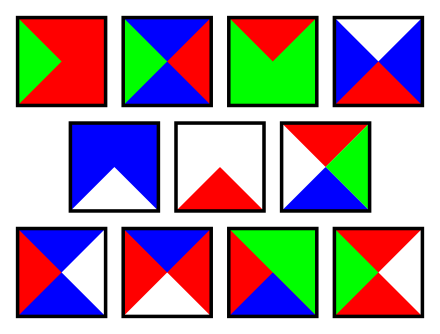
\includegraphics{image_7.png}
\caption{}
\end{figure}

In 1966, Wang's student \emph{Berger }showed that there is no
\emph{general }algorithm for the Domino Problem. More formally, he
showed that the problem is \emph{undecidable} by showing that it is
computationally \emph{isomorphic }to the \emph{halting problem }(the
first problem ever shown to be undecidable, by Turing). However, there
could be tiling-problem algorithms for subsets of the \emph{set of all
tile sets }(for example, the* Conway criterion*) and some still search
for them today.

Heesch's Problem and \emph{Heesch numbers }were devised to help with the
creation of such an algorithm for single tiles and to give a
quantitative indication of the extent to which a tile does or doesn't
tessellate. The Heesch number of a tile is the maximum number of layers
of clones that can completely surround the previous layer's perimeter
and the eponymous problem is to determine precisely the set of numbers
that \emph{can be Heesch numbers. }To illustrate what this means,
consider a regular pentagon's Heesch number: 1.

\begin{figure}[htbp]
\centering
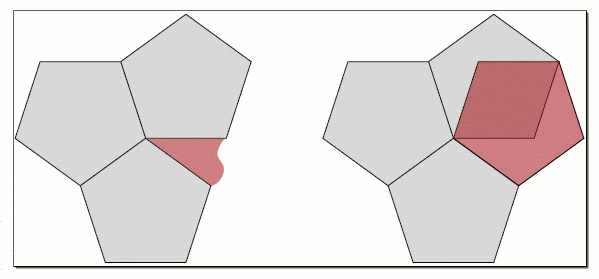
\includegraphics{image_8.gif}
\caption{}
\end{figure}

This is because the 2nd layer would have to touch the sides inside the
cracks between the pentagons of the first layer (commonly referred to as
the first \emph{corona}), which is clearly impossible. Also, the
tessellating regular polygons first mentioned in this article trivially
have a Heesch number of .

Can we have a tile of finite Heesch number? It appears so: in 1995,
Robert Ammann found a tile of Heesch number 3 and also constructed a
tile, using indentations and projections on sides of hexagons, of Heesch
number 4 and subsequently Casey Mann found an infinite family of tiles
of Heesch number \emph{5}, which is the highest finite number known to
date.

\begin{figure}[htbp]
\centering
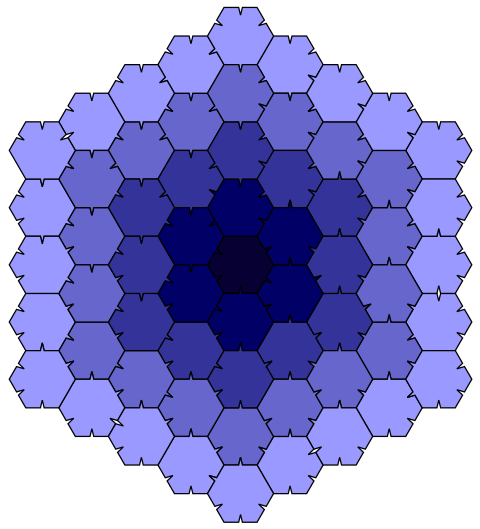
\includegraphics{image_9.png}
\caption{}
\end{figure}

You can see in the image that in the outermost layer there are four
cases where indents in the hexagons ``touch'' each other -- these parts
of the perimeter cannot be covered in the next layer, giving the
adjusted hexagon a Heesch number of 4.

The idea of the Heesch problem is to see whether there is a maximum
Heesch number . If this was true then you could construct a finite
tiling-problem algorithm: simply attempt to surround it by itself times
and if you can clearly continue then its Heesch number must be infinite,
thus proving that it tessellates. This algorithm wouldn't be
particularly efficient (at minimum, it would be an EXPTIME, potentially
even EXPTIME-complete, algorithm for those who are of the
\emph{computational complexity} persuasion) but it would represent a
great step forward.

This demonstrates one of the remarkable facts about tiling as a subject
to study: it is so simple to explain \& to think about and yet its
problems are apparently so difficult. Beyond using rational thought,
having a good understanding of geometry and perhaps studying others'
work, there are no generally accepted tools or techniques used to solve
tiling problems. The majority of those who have moved the subject
forward have been individuals looking into the topic as a hobby.

If you've found this article interesting (or you just enjoy gazing at
beautiful tilings), we suggest these topics for further reading:

\begin{itemize}
\item
  Roger Penrose's contribution to aperiodic tilings
\item
  Wikipedia's wonderful catalog of \emph{Euclidean tilings by convex
  regular polygons}
\item
  Golden Triangles
\item
  \emph{The trouble with five }by Cambridge's \emph{Plus Magazine.}
\item
  Voronoi tesselations
\end{itemize}

\subsection{Challenge I.:}\label{challenge-i.}

\textbf{a) }The \emph{five-fold symmetry problem }is to find a tile set
that consists of polygons with exactly five-fold symmetry or to show
that such a set cannot exist. Your goal is much simpler, though themed
on that basis: \textbf{Find one or more irregular pentagons that tile.}

\textbf{b) Find a prototile/shape of Heesch number 3. }This is much
harder, and we don't have the answer to this, so for the purposes of
Westminster, this is an open problem!

This article was written by \emph{Isky Mathews} but feel free to send
your solutions to either columnist!
